%------------------------------------------------------------------
%	PACKAGES AND OTHER DOCUMENT CONFIGURATIONS
%------------------------------------------------------------------

\documentclass[final]{beamer}
% Default size: ARCH E1 30 x 42
\definecolor{darkblue}{HTML}{102451}

\usepackage[orientation=landscape,size=a0,scale=1]{beamerposter} % Use the beamerposter package for laying out the poster
\usepackage[utf8]{inputenc}
\usepackage[english]{babel}

\usetheme{confposter} % Use the confposter theme supplied with this template

\setbeamercolor{block title}{fg=darkblue,bg=white} % Colors of the block titles
\setbeamercolor{block body}{fg=black,bg=white} % Colors of the body of blocks
\setbeamercolor{block alerted title}{fg=white,bg=dblue!70} % Colors of the highlighted block titles
\setbeamercolor{block alerted body}{fg=black,bg=dblue!10} % Colors of the body of highlighted blocks
% Many more colors are available for use in beamerthemeconfposter.sty

%-----------------------------------------------------------
% Define the column widths and overall poster size
% To set effective sepwid, onecolwid and twocolwid values, first choose how many columns you want and how much separation you want between columns
% In this template, the separation width chosen is 0.024 of the paper width and a 4-column layout
% onecolwid should therefore be (1-(# of columns+1)*sepwid)/# of columns e.g. (1-(4+1)*0.024)/4 = 0.22
% Set twocolwid to be (2*onecolwid)+sepwid = 0.464
% Set threecolwid to be (3*onecolwid)+2*sepwid = 0.708

\newlength{\sepwid}
\newlength{\onecolwid}
\newlength{\twocolwid}
\newlength{\threecolwid}
\setlength{\paperwidth}{42in} % A0 width: 46.8in
\setlength{\paperheight}{32in} % A0 height: 33.1in
\setlength{\sepwid}{0.024\paperwidth} % Separation width (white space) between columns
\setlength{\onecolwid}{0.295\paperwidth} % Width of one column
\setlength{\twocolwid}{0.464\paperwidth} % Width of two columns
\setlength{\threecolwid}{0.708\paperwidth} % Width of three columns
\setlength{\topmargin}{-0.5in} % Reduce the top margin size
\setlength\labelsep{\dimexpr\labelsep + 1em\relax}
\setlength{\parskip}{0.5\baselineskip}
\setlength{\parindent}{0em}

%-----------------------------------------------------------
% \renewcommand{\figurename}{Fig.}

\usepackage{caption}
\captionsetup{labelformat=simple, labelsep=colon}

\usepackage{graphicx}  % Required for including images

\usepackage{booktabs} % Top and bottom rules for tables

\usepackage{bbm} % more BB
\input{\string~/HeadRs/common_supplement.tex}

\usepackage{array}
\newcommand{\PreserveBackslash}[1]{\let\temp=\\#1\let\\=\temp}
\newcolumntype{C}[1]{>{\PreserveBackslash\centering}p{#1}}
\newcolumntype{R}[1]{>{\PreserveBackslash\raggedleft}p{#1}}
\newcolumntype{L}[1]{>{\PreserveBackslash\raggedright}p{#1}}

\usepackage{multicol}

\usepackage{adjustbox}
\usepackage{pgf}
\usepackage{pgfplots}
\usepackage{cmbright}
\pgfplotsset{compat=1.17}
\usepackage{tikz}
\usetikzlibrary{graphs, arrows.meta, automata, positioning, decorations}

\usepackage[sorting=none]{biblatex}
\renewcommand*{\bibfont}{\footnotesize}
\addbibresource{ser_poster.bib}

% -----------------------------------------------------------
\setbeamertemplate{headline}{
 \leavevmode
  \begin{columns}
   \begin{column}{\linewidth} % line
    \vskip1cm
    \centering
    \usebeamercolor{title in headline}{\color{jblue}
        \Huge % CHANGE this line for the size of the title
        {\textbf{\inserttitle}}\\[0.5ex]}
    \usebeamercolor{author in headline}{\color{fg}
        \Large % CHANGE this line for the size of the author
        {\insertauthor}\\[1ex]}
    \usebeamercolor{institute in headline}{\color{fg}
        \large % CHANGE this line for the size of the institut
        {\insertinstitute}\\[1ex]}
    \vskip1cm
   \end{column}
   \vspace{1cm}
  \end{columns}
 \vspace{0.5in} % CHANGE this line for the space between your title and the horizontal rule
 \begin{beamercolorbox}[wd=46in,colsep=0.1cm]{cboxb}\end{beamercolorbox}
 \vspace{0.1in} % CHANGE this line for the space between your horizontal rule and your main body
}

%------------------------------------------------------------------
%	TITLE SECTION
%------------------------------------------------------------------
\title{\huge Evaluating Exposure Limits for Reducing Non-Hodgkin Lymphoma Incidence\\[-0.25\baselineskip]{\Large An Application of the Hazard-Extended Iterative Conditional Expectation G-formula}} % Poster title
\author{Kevin T. Chen\textsuperscript{\small 1,2}, Ellen A. Eisen\textsuperscript{\small 1}} % Author(s)
\institute{
	University of California, Berkeley School of Public Health\\
	\normalsize
	\textsuperscript{1} Division of Environmental Health Sciences
	\hspace{1em}
	\textsuperscript{2} Division of Epidemiology \& Biostatistics
} % Institution(s)
%------------------------------------------------------------------

\begin{document}

% add logo
\addtobeamertemplate{headline}{}
{\begin{tikzpicture}[remember picture, overlay]
			\node [anchor=north west, inner sep=2.25cm]  at (current page.north west)
			{
\includegraphics[height=10cm]{ucberkeleyseal_139_540.eps}};
  \end{tikzpicture}}

\addtobeamertemplate{block end}{}{\vspace*{2ex}} % White space under blocks
\addtobeamertemplate{block alerted end}{}{\vspace*{2ex}} % White space under highlighted (alert) blocks

\setlength{\belowcaptionskip}{2ex} % White space under figures
\setlength\belowdisplayshortskip{2ex} % White space under equations

\setlength{\leftmargini}{\baselineskip}
\setlength{\leftmarginii}{\baselineskip}

\begin{frame}[t] % The whole poster is enclosed in one beamer frame

\begin{columns}[t,onlytextwidth,totalwidth=\onecolwid]


\begin{column}{\sepwid}\end{column} % Empty spacer column

\begin{column}{\onecolwid} % The first column

%------------------------------------------------------------------
%	Introduction
%------------------------------------------------------------------


\begin{block}{Introduction}

\begin{minipage}{\linewidth}\begin{itemize}\setlength{\itemsep}{7pt}
\item Non-Hodgkin lymphoma (NHL) incidence increased 4-fold since 1960 \nocite{Ekstrom-Smedby_2006}
\item Rise in NHL followed growing use of industrial chemicals
\item Past occupational studies of NHL were limited
 	\begin{itemize}\setlength{\itemsep}{7pt}\normalsize
	\item Crude exposure assessment
	\item Conditional estimates of association
	\item Unrealistic static interventions
	\item Potential bias due to the healthy worker survivor effect (HWSE) \nocite{Arrighi_1994}
	\end{itemize}
\item \bfseries We estimate counterfactual cumulative incidence of NHL from 1985 to 2004 under hypothetical limits on average annual occupational exposure to metalworking fluid (MWF)
\end{itemize}
\end{minipage}

\end{block}

%------------------------------------------------------------------
%	Methods
%------------------------------------------------------------------

\begin{block}{Methods}

\textbf{Interventions:} $g_a$ on average exposure $A_k$ in year $k$:

$$g_a:\ A_k \longrightarrow
\begin{cases}
A_k & \text{if } A_k \le a \\
a & \text{if } A_k > a \\
\end{cases}$$

\begin{itemize}\setlength{\itemsep}{7pt}
\item Hypothetical limits: $a = 0.5,\ 0.25,\ 0.05$ mg/m\textsuperscript{3}
\item $g_a$ is a longitudinal stochastic intervention
\item No censoring by death
\end{itemize}

\vspace{0.5\baselineskip}\textbf{Data: United Auto Workers-General Motors Cohort Study}

\vspace{0.5\baselineskip}
\begin{minipage}{\linewidth}
\begin{itemize}\setlength{\itemsep}{7pt}
\item \textit{Quantitative exposure} for each person-year of employment from hire to 1995 based on several hundred samples
\item \textit{NHL outcome} from 1985 to 2005 via linkage to the Michican Cancer Registry (MCR) and the Surveillance, Epidemiology, and End Results (SEER) Program
\item \textit{Covariates} are age, calendar year, employment status, cumulative time off, year of hire, sex, race, and plant
\end{itemize}
\end{minipage}\vspace{0.25\baselineskip}



\vspace{0.5\baselineskip}\textbf{Estimation: Hazard-extended parametric G-formula \nocite{Wen_2020}}

\begin{itemize}\setlength{\itemsep}{7pt}
\item Pooling exposure history over $K = 8$ time periods
\item Exposure history at each time summmarized as cumulative exposure
\end{itemize}

\vspace{0.5\baselineskip}\textbf{Assumptions for causal inference}
\vspace{0.5\baselineskip}

\begin{minipage}{\linewidth}
\begin{itemize}\setlength{\itemsep}{7pt}
\item \textit{Conditional exchangeability}
\item \textit{Positivity (overlap)}
\item \textit{Consistency}
\item \textit{Correct model specification}
\end{itemize}
\end{minipage}\vspace{0.25\baselineskip}

\end{block}

\end{column} % End of the first column

\begin{column}{\sepwid}\end{column} % Empty spacer column

\begin{column}{\onecolwid} % Begin a column which is two columns wide (column 2)

%------------------------------------------------------------------
%	Results
%------------------------------------------------------------------
\begin{block}{Results}

\begin{table}\renewcommand{\arraystretch}{1.1}
\caption{\bfseries Population and non-Hodgkin lymphoma (NHL) case characteristics.}
\small
\begin{tabular}{p{0.4\linewidth}rlcrl}
  \toprule
 & \multicolumn{2}{c}{Study population} 	&  & \multicolumn{2}{c}{NHL cases} \\
  \midrule
	$N$ (person-years) & 34,734 & (596,698) &  & 231 & (2,777) \\
  Race &  &  &  &  &  \\
  \hspace{1em}White & 22,789 & (66\%) 		&  & 173 & (75\%) \\
  \hspace{1em}Black & 6,304 & (18\%) 			&  & 21 & (9\%) \\
  \hspace{1em}Unknown & 5,641 & (16\%) 		&  & 37 & (16\%) \\
  Sex &  &  &  &  &  \\
  \hspace{1em}Male & 30,235 & (87\%)		 	&  & 206 & (89\%) \\
  \hspace{1em}Female & 4,499 & (13\%) 		&  & 25 & (11\%) \\
  Plant &  &  &  &  &  \\
  \hspace{1em}Plant 1 & 8,721 & (25\%) 		&  & 68 & (29\%) \\
  \hspace{1em}Plant 2 & 14,258 & (41\%) 	&  & 90 & (39\%) \\
  \hspace{1em}Plant 3 & 11,755 & (34\%) 	&  & 73 & (32\%) \\
  Ever exposed$^1$
											& 31,044 & (89\%) 	&  & 210 & (91\%) \\
	Deceased by end of follow-up
																					& 10,384 & (30\%) 	&  & 33 & (14\%) \\
  \hline
  Year of birth & 1940 & (1925, 1950) 		&  & 1929 & (1919, 1940) \\
  Year of hire & 1967 & (1953, 1976) 			&  & 1959 & (1951, 1969) \\
  Age at hire (years) & 23.6 & (20.0, 30.1)					 		&  & 25.4 & (21.1, 33.6) \\
	Cumulative time off (years)$^1$ & 1.05 & (0.30, 1.80) &  & 0.71 & (0.14, 1.40) \\
  Years at work$^2$ & 15.3 & (7.3, 27.1) 								&  & 19.2 & (8.0, 29.9) \\
  Cumulative exposure (mg/m$^2\cdot$yr)$^{1,3}$
							& 4.65 & (1.85, 12.13) 					&  & 7.16 & (2.86, 20.91) \\
	\midrule
	\multicolumn{6}{p{0.85\linewidth}}{
	$^1$ Lagged 10 years; $^2$ Among those who left work before 1995;}\\
	\multicolumn{6}{p{0.85\linewidth}}{
	$^3$ Among ever-exposed indidivuals.}\\
   \bottomrule
	\end{tabular}
\end{table}

\vspace{1em}


% \begin{figure}
% \caption{foo.}
% \begin{center}
% \begin{tikzpicture}[>={Stealth[scale=1.3]}, auto,
% semithick, scale=6,
% thick, fill=white, inner sep=0pt, minimum size=0pt]
% \tikzstyle{every state}=[
% shape = rectangle, align = center, draw = none
% ]
% %
% \node[state] at (0, 2.5) (L0) {$L_{k-1}$};
% \node[state] at (1.5, 2.5) (L1) {$L_{k}$};
% \node[state] at (3, 2.5) (L2) {$L_{k + 1}$};
% \node[state] at (0.6, 1.66) (A0) {$A_{k-1}$};
% \node[state] at (2.1, 1.66) (A1) {$A_{k}$};
% \node[state] at (3.6, 1.66) (A2) {$A_{k + 1}$};
% \node[state] at (1.2, 0.833) (C0) {$C_{k-1}$};
% \node[state] at (2.7, 0.833) (C1) {$C_{k}$};
% \node[state] at (4.2, 0.833) (C2) {$C_{k + 1}$};
% \node[state] at (1.8, 0) (Y0) {$Y_{k-1}$};
% \node[state] at (3.3, 0) (Y1) {$Y_{k}$};
% \node[state] at (4.8, 0) (Y2) {$Y_{k + 1}$};
% %
% \path[->] (L0) edge (A0);
% \path[->] (L0) edge [bend right=40] (C0);
% \path[->] (L0) edge [bend right=40] (Y0);
% \path[->] (L0) edge (L1);
% \path[->] (A0) edge (C0);
% \path[->] (A0) edge [bend right=40] (Y0);
% \path[->] (A0) edge (L1);
% \path[->] (A0) edge (A1);
% \path[->] (A0) edge (C1);
% \path[->] (C0) edge (Y0);
% \path[->] (C0) edge (L1);
% \path[->] (C0) edge (A1);
% \path[->] (C0) edge (C1);
% \path[->] (Y0) edge (L1);
% \path[->] (Y0) edge (A1);
% \path[->] (Y0) edge (C1);
% \path[->] (Y0) edge (Y1);
% %
% \path[->] (L1) edge (A1);
% \path[->] (L1) edge [bend right=40] (C1);
% \path[->] (L1) edge [bend right=40] (Y1);
% \path[->] (L1) edge (L2);
% \path[->] (A1) edge (C1);
% \path[->] (A1) edge [bend right=40] (Y1);
% \path[->] (A1) edge (L2);
% \path[->] (A1) edge (A2);
% \path[->] (A1) edge (C2);
% \path[->] (C1) edge (Y1);
% \path[->] (C1) edge (L2);
% \path[->] (C1) edge (A2);
% \path[->] (C1) edge (C2);
% \path[->] (Y1) edge (L2);
% \path[->] (Y1) edge (A2);
% \path[->] (Y1) edge (C2);
% \path[->] (Y1) edge (Y2);
% %
% %
% \path[->] (L2) edge (A2);
% \path[->] (L2) edge [bend right=40] (C2);
% \path[->] (L2) edge [bend right=40] (Y2);
% \path[->] (A2) edge (C2);
% \path[->] (A2) edge [bend right=40] (Y2);
% \path[->] (C2) edge (Y2);
% \end{tikzpicture}
% \end{center}
% \end{figure}

\begin{figure}
\caption{\bfseries Cumulative exposure at end of follow-up under hypothetical limits on average annual exposure. Rug plots mark cumulative exposure accrued by NHL cases at end of follow-up.}
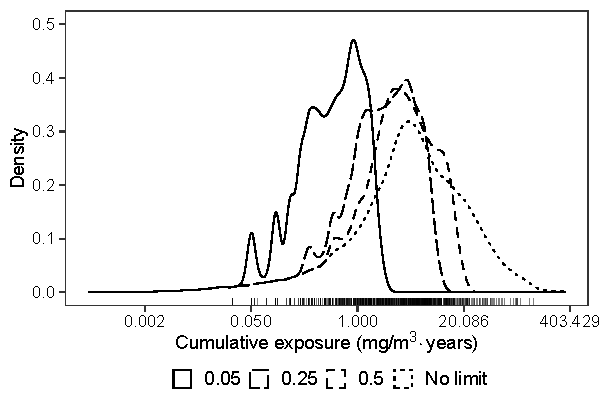
\includegraphics[width=0.87\linewidth]{../../../resources/shift-soluble.pdf}
\end{figure}

\end{block}

\end{column} % End of column 2

\begin{column}{\sepwid}\end{column}

\begin{column}{\onecolwid}

\begin{figure}
\caption{\bfseries Counterfactual cumulative incidence ratio estimates comparing hypothetical limits on average annual exposure to no limit.}
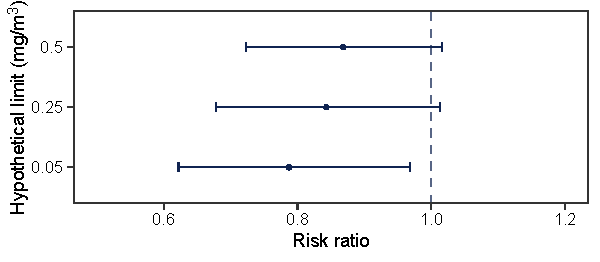
\includegraphics[width=0.87\linewidth]{resources/rr.pdf}
\end{figure}

\begin{table}\renewcommand{\arraystretch}{1.1}
\caption{\bfseries Counterfactual cumulative incidence estimates under hypothetical limits on average annual exposure and no censoring.}
\small
\begin{tabular}{p{0.17\linewidth}C{0.2\linewidth}cC{0.11\linewidth}C{0.2\linewidth}}
\toprule
Exposure limit
	& \thead{Person-years\\intervened (\%)}
	&& \thead{Cases\\expected}
	& (95\% BS CI)
	%& RR & (95\% BS CI)
	 \\ \midrule
None & 0 && 332 & (283, 378) %& 1.00 &
 \\
 0.5\phantom{0} mg/m\textsuperscript{3} & 23.8 && 288 & (226, 354)
 % & 0.87 & (0.72, 1.02)
  \\
0.25 mg/m\textsuperscript{3} & 36.2 && 280 & (214, 353)
 % & 0.84 & (0.68, 1.01)
 \\
0.05 mg/m\textsuperscript{3} & 43.9 && 261 & (199, 330)
 % & 0.79 & (0.62, 0.97)
\\
\bottomrule
\end{tabular}
\end{table}

\vspace{0.5em}

%------------------------------------------------------------------
%	Discussion
%------------------------------------------------------------------

\begin{block}{Discussion and Conclusions}

\begin{itemize}\setlength{\itemsep}{7pt}
\item Limiting average annual MWF exposure reduces NHL incidence
\item Longitudinal stochastic interventions represent realistic policies
	\begin{itemize}\setlength{\itemsep}{7pt}\normalsize
	\item NIOSH Recommended Exposure Limit is 0.5 mg/m\textsuperscript{3} \nocite{NIOSH_1998}
	\end{itemize}
\item Our method reduced potential bias due to HWSE
\item Outcome models were logistic regressions; assumption of correct model specification may be more plausible under machine learning approaches with cross-validation
\end{itemize}

\end{block}

\vspace*{-0.5\baselineskip}

%------------------------------------------------------------------
%	References
%------------------------------------------------------------------

\begin{block}{References}
		\setlength{\bibitemsep}{0pt}
    \printbibliography
\end{block}

\vspace*{-0.5\baselineskip}

%------------------------------------------------------------------
%	Acknowledgement of support
%------------------------------------------------------------------

\begin{block}{Acknowledgement of support}
This poster was supported by Training Grant T42OH008429, funded by the National Institute for Occupational Safety and Health (NIOSH) / Centers for Disease Control and Prevention (CDC)
\end{block}

\vspace*{-1\baselineskip}

\end{column} % End of column 3

\begin{column}{\sepwid}\end{column}% Empty spacer column

\end{columns} % End of all the columns in the poster

\end{frame} % End of the enclosing frame

\end{document}
